\begin{figure}[h]
    \centering
    
    % RESCAL (a)
    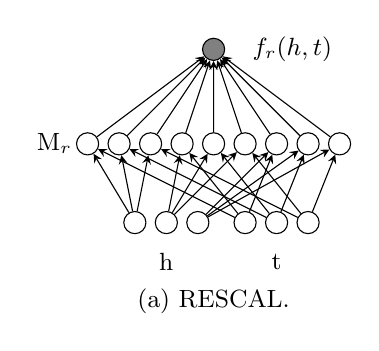
\begin{tikzpicture}[
        neuron/.style={circle, draw, fill=white, minimum size=8pt, inner sep=0pt},
        output/.style={circle, draw, fill=gray, minimum size=8pt, inner sep=0pt},
        connection/.style={-stealth, thin},
        label/.style={font=\small}
    ]
        % Input layer h (left)
        \foreach \i in {1,2,3} {
            \node[neuron] (h\i) at (\i*0.4 - 0.4, -1) {};
        }
        \node[label] at ([yshift=-0.5cm]h2) {h};
        
        % Input layer t (right)  
        \foreach \i in {1,2,3} {
            \node[neuron] (t\i) at (\i*0.4 + 1, -1) {};
        }
        \node[label] at ([yshift=-0.5cm]t2) {t};
        
        % Hidden layer Mr
        \foreach \i in {1,2,3,4,5,6,7,8,9} {
            \node[neuron] (mr\i) at (\i*0.4 - 1, 0) {};
        }
        \node[label] at ([xshift=-12pt]mr1) {M$_r$};
        
        % Output
        \node[output] (out1) at (1, 1.2) {};
        \node[label] at ([xshift=1cm]out1) {$f_r(h,t)$};
        
        % Connections from h to Mr
        \foreach \i in {1,2,3} {
            \foreach \j in {1,2,3} {
                \pgfmathtruncatemacro{\target}{(\i-1)*3+\j}
                \draw[connection] (h\i) -- (mr\target);
            }
        }
        
        % Connections from t to Mr
        \foreach \i in {1,2,3} {
            \foreach \j in {1, 2, 3} {
                \pgfmathtruncatemacro{\target}{\i + ((\j - 1) * 3)}
                \draw[connection] (t\i) -- (mr\target);
            }
        }
        
        % Connections from Mr to output
        \foreach \i in {1,2,3,4,5,6,7,8,9} {
            \draw[connection] (mr\i) -- (out1);
        }
        
        % Label
        \node[label] at (1, -2) {(a) RESCAL.};
    \end{tikzpicture}
    \hspace{1cm}
    % DistMult (b)
    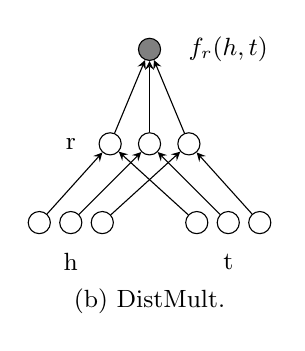
\begin{tikzpicture}[
        neuron/.style={circle, draw, fill=white, minimum size=8pt, inner sep=0pt},
        output/.style={circle, draw, fill=gray, minimum size=8pt, inner sep=0pt},
        connection/.style={-stealth, thin},
        label/.style={font=\small}
    ]
        % Input layer h (left)
        \node[label] (h_label) at (0, -1.5) {h};
        \foreach \i in {1,2,3} {
            \pgfmathsetmacro{\target}{(\i-2)*0.4}
            \node[neuron] (h2\i) at ([xshift=\target cm, yshift=0.5cm]h_label) {};
        }
        
        % Input layer t (right)
        \node[label] (t_label) at (2, -1.5) {t};
        \foreach \i in {1,2,3} {
            \pgfmathsetmacro{\target}{(\i-2)*0.4}
            \node[neuron] (t2\i) at ([xshift=\target cm, yshift=0.5cm]t_label) {};
        }
        
        % Hidden layer r
        \foreach \i in {1,2,3} {
            \node[neuron] (r2\i) at (0.5*\i, 0) {};
        }
        \node[label] at ([xshift=-0.5cm]r21) {r};
        
        % Output
        \node[output] (out2) at (1, 1.2) {};
        \node[label] at ([xshift=1cm]out2) {$f_r(h,t)$};
        
        % Connections - element-wise multiplication pattern
        \foreach \i in {1,2,3} {
            \draw[connection] (h2\i) -- (r2\i);
            \draw[connection] (t2\i) -- (r2\i);
            \draw[connection] (r2\i) -- (out2);
        }
        
        % Label
        \node[label] at (1, -2) {(b) DistMult.};
    \end{tikzpicture}
    \hspace{1cm}
    % HolE (c)
    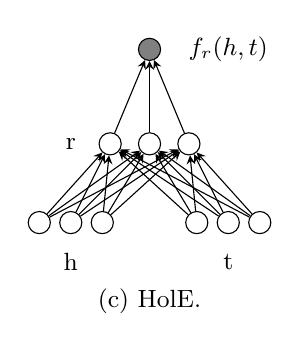
\begin{tikzpicture}[
        neuron/.style={circle, draw, fill=white, minimum size=8pt, inner sep=0pt},
        output/.style={circle, draw, fill=gray, minimum size=8pt, inner sep=0pt},
        connection/.style={-stealth, thin},
        label/.style={font=\small}
    ]
        % Input layer h (left)
        \node[label] (h_label) at (0, -1.5) {h};
        \foreach \i in {1,2,3} {
            \pgfmathsetmacro{\target}{(\i-2)*0.4}
            \node[neuron] (h3\i) at ([xshift=\target cm, yshift=0.5cm]h_label) {};
        }
        
        % Input layer t (right)
        \node[label] (t_label) at (2, -1.5) {t};
        \foreach \i in {1,2,3} {
            \pgfmathsetmacro{\target}{(\i-2)*0.4}
            \node[neuron] (t3\i) at ([xshift=\target cm, yshift=0.5cm]t_label) {};
        }
        
        % Hidden layer r
        \foreach \i in {1,2,3} {
            \node[neuron] (r3\i) at (0.5*\i, 0) {};
        }
        \node[label] at ([xshift=-0.5cm]r31) {r};
        
        % Output
        \node[output] (out3) at (1, 1.2) {};
        \node[label] at ([xshift=1cm]out3) {$f_r(h,t)$};
        
        % Connections - circular correlation pattern (more complex)
        \foreach \i in {1,2,3} {
            \foreach \j in {1,2,3} {
                \draw[connection] (h3\i) -- (r3\j);
                \draw[connection] (t3\i) -- (r3\j);
            }
        }
        
        % Connections from r to output
        \foreach \i in {1,2,3} {
            \draw[connection] (r3\i) -- (out3);
        }
        
        % Label
        \node[label] at (1, -2) {(c) HolE.};
    \end{tikzpicture}
    
    \caption{Simple illustrations of semantic matching models RESCAL, DistMult, and HolE \parencite{ZHANG2024123876}.}
    \label{fig:semantic_maching_models}
\end{figure}